\documentclass{mini}
\usepackage[utf8]{inputenc}
\usepackage[polish]{babel}
\usepackage{enumitem}
\usepackage{todonotes}
\presetkeys
	{todonotes}
	{inline}{}

%------------------------------------------------------------------------------%
\title{Linux w Systemach Wbudowanych}
\author{Karol Dzitkowski}
\monthyear{\today}
%------------------------------------------------------------------------------%

\usepackage{listings}
\usepackage{graphicx}

\begin{document}
\maketitle
\tableofcontents
\newpage

\section{Treść zadania}
\begin{enumerate}
\item Przygotować „administracyjny” system Linux pracujący w 
initramfs, umożliwiający przygotowanie karty pamięci SD do 
instalacji systemu Linux pracującego z systemem plików 
e2fs, montowanym z partycji 2 na karcie SD
\item Przygotować „użytkowy” system Linux pracujący z 
systemem plików e2fs, zawierający serwer WWW, 
udostępniający pliki z partycji 3 na karcie SD i umożliwiający 
wgrywanie nowych plików po podaniu hasła.
\item Należy też przygotować bootloader, umożliwiający 
określenie (przy pomocy przycisku), który system ma zostać 
załadowany.
\end{enumerate}

\section{Rozwiązanie}
Stworzyłem system na podstawie systemu 3 mający dwie wersje systemu linux używając buildroota. 
Bazując na rozwiązaniu zadania 3 rozbudowałem oba systemy o możliwość używania sieci wifi do
połączenia z siecią instalując odpowiednie sterowniki i modysikując pliki systemowe. Dodatkowo
rozbudowałem serwer www w systemie użytkownika o możliwość bardziej zaawansowanego wgrywania
plików mp3 i ich odtwarzania na użądzeniu podłączonym do raspberry za pomocą złącza JACK.
Urządzenie korzysta z karty wifi pod USB firmy Pentagram (Ralink rt2780). System użytkownika
umożliwia również udostępnienie funkcji AirPlay do odtwarzania muzyki dla urządzeń Apple.

\subsection{Konfiguracja \emph{buildroot}}
Bazuję na konfiguracji z zadania trzeciego i dodatkowo w menu wywołanym za pomocą komendy:

\begin{lstlisting}[language=bash]
make menuconfig
\end{lstlisting}	

Dla systemu użytkownika ustawiam:
\begin{enumerate}
\item Kernel $\rightarrow$ Configuration file path $\rightarrow$ ustawiam na \emph{.linux-config} w celu łatwiejszego utrzymywania konfiguracji jądra
\item Build options $\rightarrow$ wyłączam opcję ,,Build packages with debugging symbols''
\item Target Packages $\rightarrow$ Hardware handling $\rightarrow$ Firmware $\rightarrow$ Wifi firmware $\rightarrow$ ustawiam opcję Ralink rt27xx/rt28xx/rt30xx na włączoną $[*]$ oraz po drodze upewniam się ze opcja rpi-firmware jest włączona (w opcjach Firmware).
\item System configuration $\rightarrow$ /dev management $\rightarrow$ ustawiam Dynamic using eudev (Root filesystem overlay directories powinno być ustawione na folder overlay w moim przypadku na \emph{moje})
\item Target Packages $\rightarrow$ Audio and video applications $\rightarrow$ wybieram alsa-utils oraz mpg123 
\item Target Packages $\rightarrow$ Libraries $\rightarrow$ Audio/Sound $\rightarrow$ wybieram alsa-lib z wszystkimi bibliotekami (u mnie było to domyślnie)
\item Target Packages $\rightarrow$ Libraries $\rightarrow$ Networking $\rightarrow$ wybieram libshairplay (do AirPlay)
\item Target Packages $\rightarrow$ Networking applications $\rightarrow$ wybieram avahi, wpa\_supplicant (ze wszystkimi opcjami) oraz shairport-sync (do AirPlay)
\end{enumerate}

Dla systemu administracyjnego ustawiam tylko opcje 1, 3, 4 i wpa\_supplicant.
Dla obu systemów należy też zmienić konfigurację jądra dodając obsługę karty sieciowej USB Ralink.

\subsection{Konfiguracja jądra}
Zmieniam konfigurację jądra wchodząc w linux-menuconfig po czym zapisuje konfigurację:
\begin{lstlisting}[language=bash]
make linux-menuconfig
cp output/build/linux-.../.config .linux-config
\end{lstlisting}	

W menu ustawiam opcje:
\begin{enumerate}
\item Networking support $\rightarrow$ Wireless $\rightarrow$ ustawienia powinny wyglądać tak:

\begin{center}
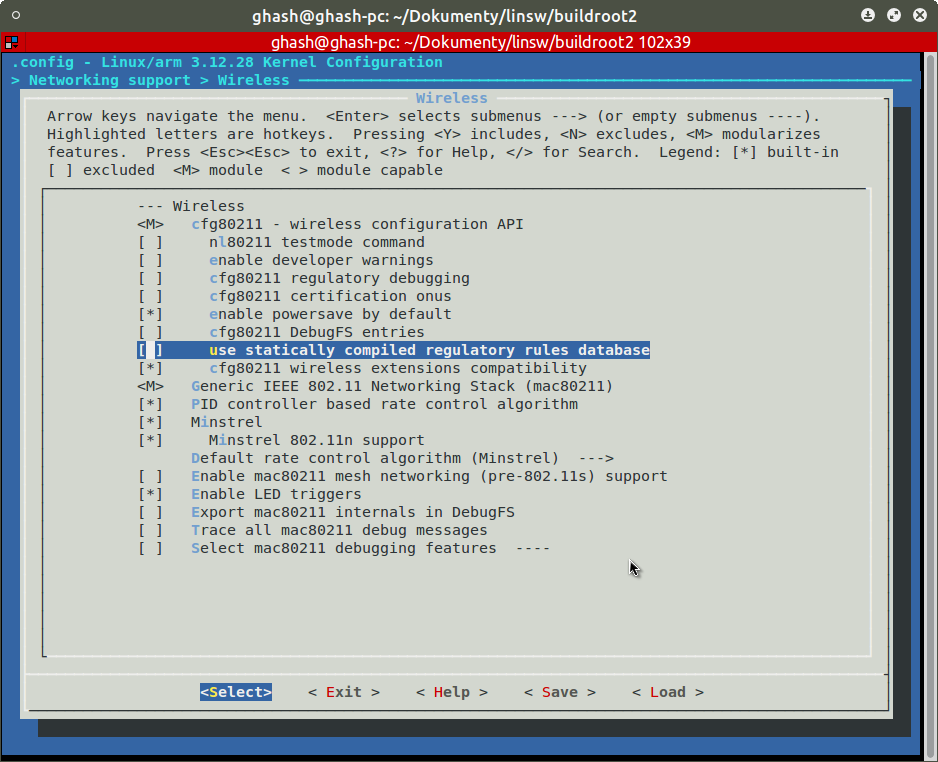
\includegraphics[width=0.5\textwidth]{NetworkingSupport_Wireless.png}
\end{center}

\item Device Drivers $\rightarrow$ Network device support $\rightarrow$ Wireless LAN $\rightarrow$ Ralink driver support $\rightarrow$ ustawienia powinny wyglądać tak:

\begin{center}
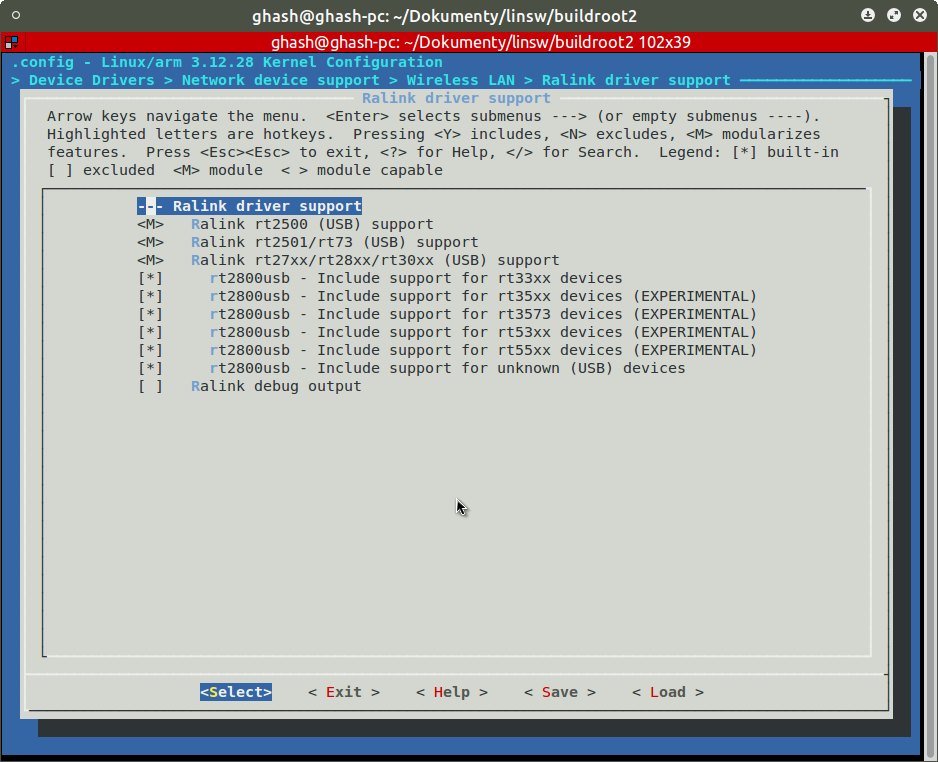
\includegraphics[width=0.5\textwidth]{DeviceDrivers.png}
\end{center}

\end{enumerate}

\section{Dostosowanie plików systemowych}
W katalogu moje w głównym katalogu buildroota tworzę strukturę plików która nadpisze domyślną konfigurację.
Robię to dla obu systemów w celu automatycznego połączenia z siecią WIFI. Wygląda to następująco:
\begin{enumerate}
\item BUILDROOT/moje/etc/wpa\_supplicant.conf
\begin{lstlisting}[language=bash]
ctrl_interface=DIR=/var/run/wpa_supplicant GROUP=netdev
update_config=1
network={
ssid="<SSID SIECI WIFI>"
psk=<WYGENEROWANY PSK>
scan_ssid=1
proto=WPA RSN
key_mgmt=WPA-PSK
pairwise=CCMP TKIP
auth_alg=OPEN
}
\end{lstlisting}	
Aby wygenerować numer PSK używamy polecenia:
\begin{lstlisting}[language=bash]
wpa_passphrase "SSID SIECI WIFI" "HASLO"
\end{lstlisting}
\item BUILDROOT/moje/etc/network/interfaces
\begin{lstlisting}[language=bash]
auto lo
iface lo inet loopback
iface eth0 inet dhcp
auto wlan0
iface wlan0 inet dhcp
    wireless-essid wrt2
    pre-up wpa_supplicant -B w -D wext -i wlan0 -c /etc/wpa_supplicant.conf -dd
    post-down killall -q wpa_supplicant
\end{lstlisting}
\item BUILDROOT/moje/etc/init.d/SS99start -- z prawami do uruchomienia
\begin{lstlisting}[language=bash]
# /bin/sh
case "$1" in
	start)
		mkdir /mnt/sdcard
		mkdir /mnt/rootfs
		mount /dev/mmcblk0p1 /mnt/sdcard
		mount /dev/mmcblk0p2 /mnt/rootfs 
		;;
	stop)
		umount /dev/mmcblk0p1
		;;
	*)
		echo "Usage: $0 {start|stop}"
		exit 3 
		;;
esac
exit 0
\end{lstlisting}
\item BUILDROOT/moje/usr/bin/updateUserFs -- z prawami do uruchomienia
\begin{lstlisting}[language=bash]
#!/bin/sh
mkdir /mnt/rootfs
mount /dev/mmcblk0p2 /mnt/rootfs
cd /mnt/rootfs
rm -rf *
cd /mnt/sdcard
umount /dev/mmcblk0p2
cat rootfs.ext4 > /dev/mmcblk0p2
mount /dev/mmcblk0p2 /mnt/rootfs
resize2fs /dev/mmcblk0p2
\end{lstlisting}
\end{enumerate}


\section{Wygląd aplikacji}
\begin{center}
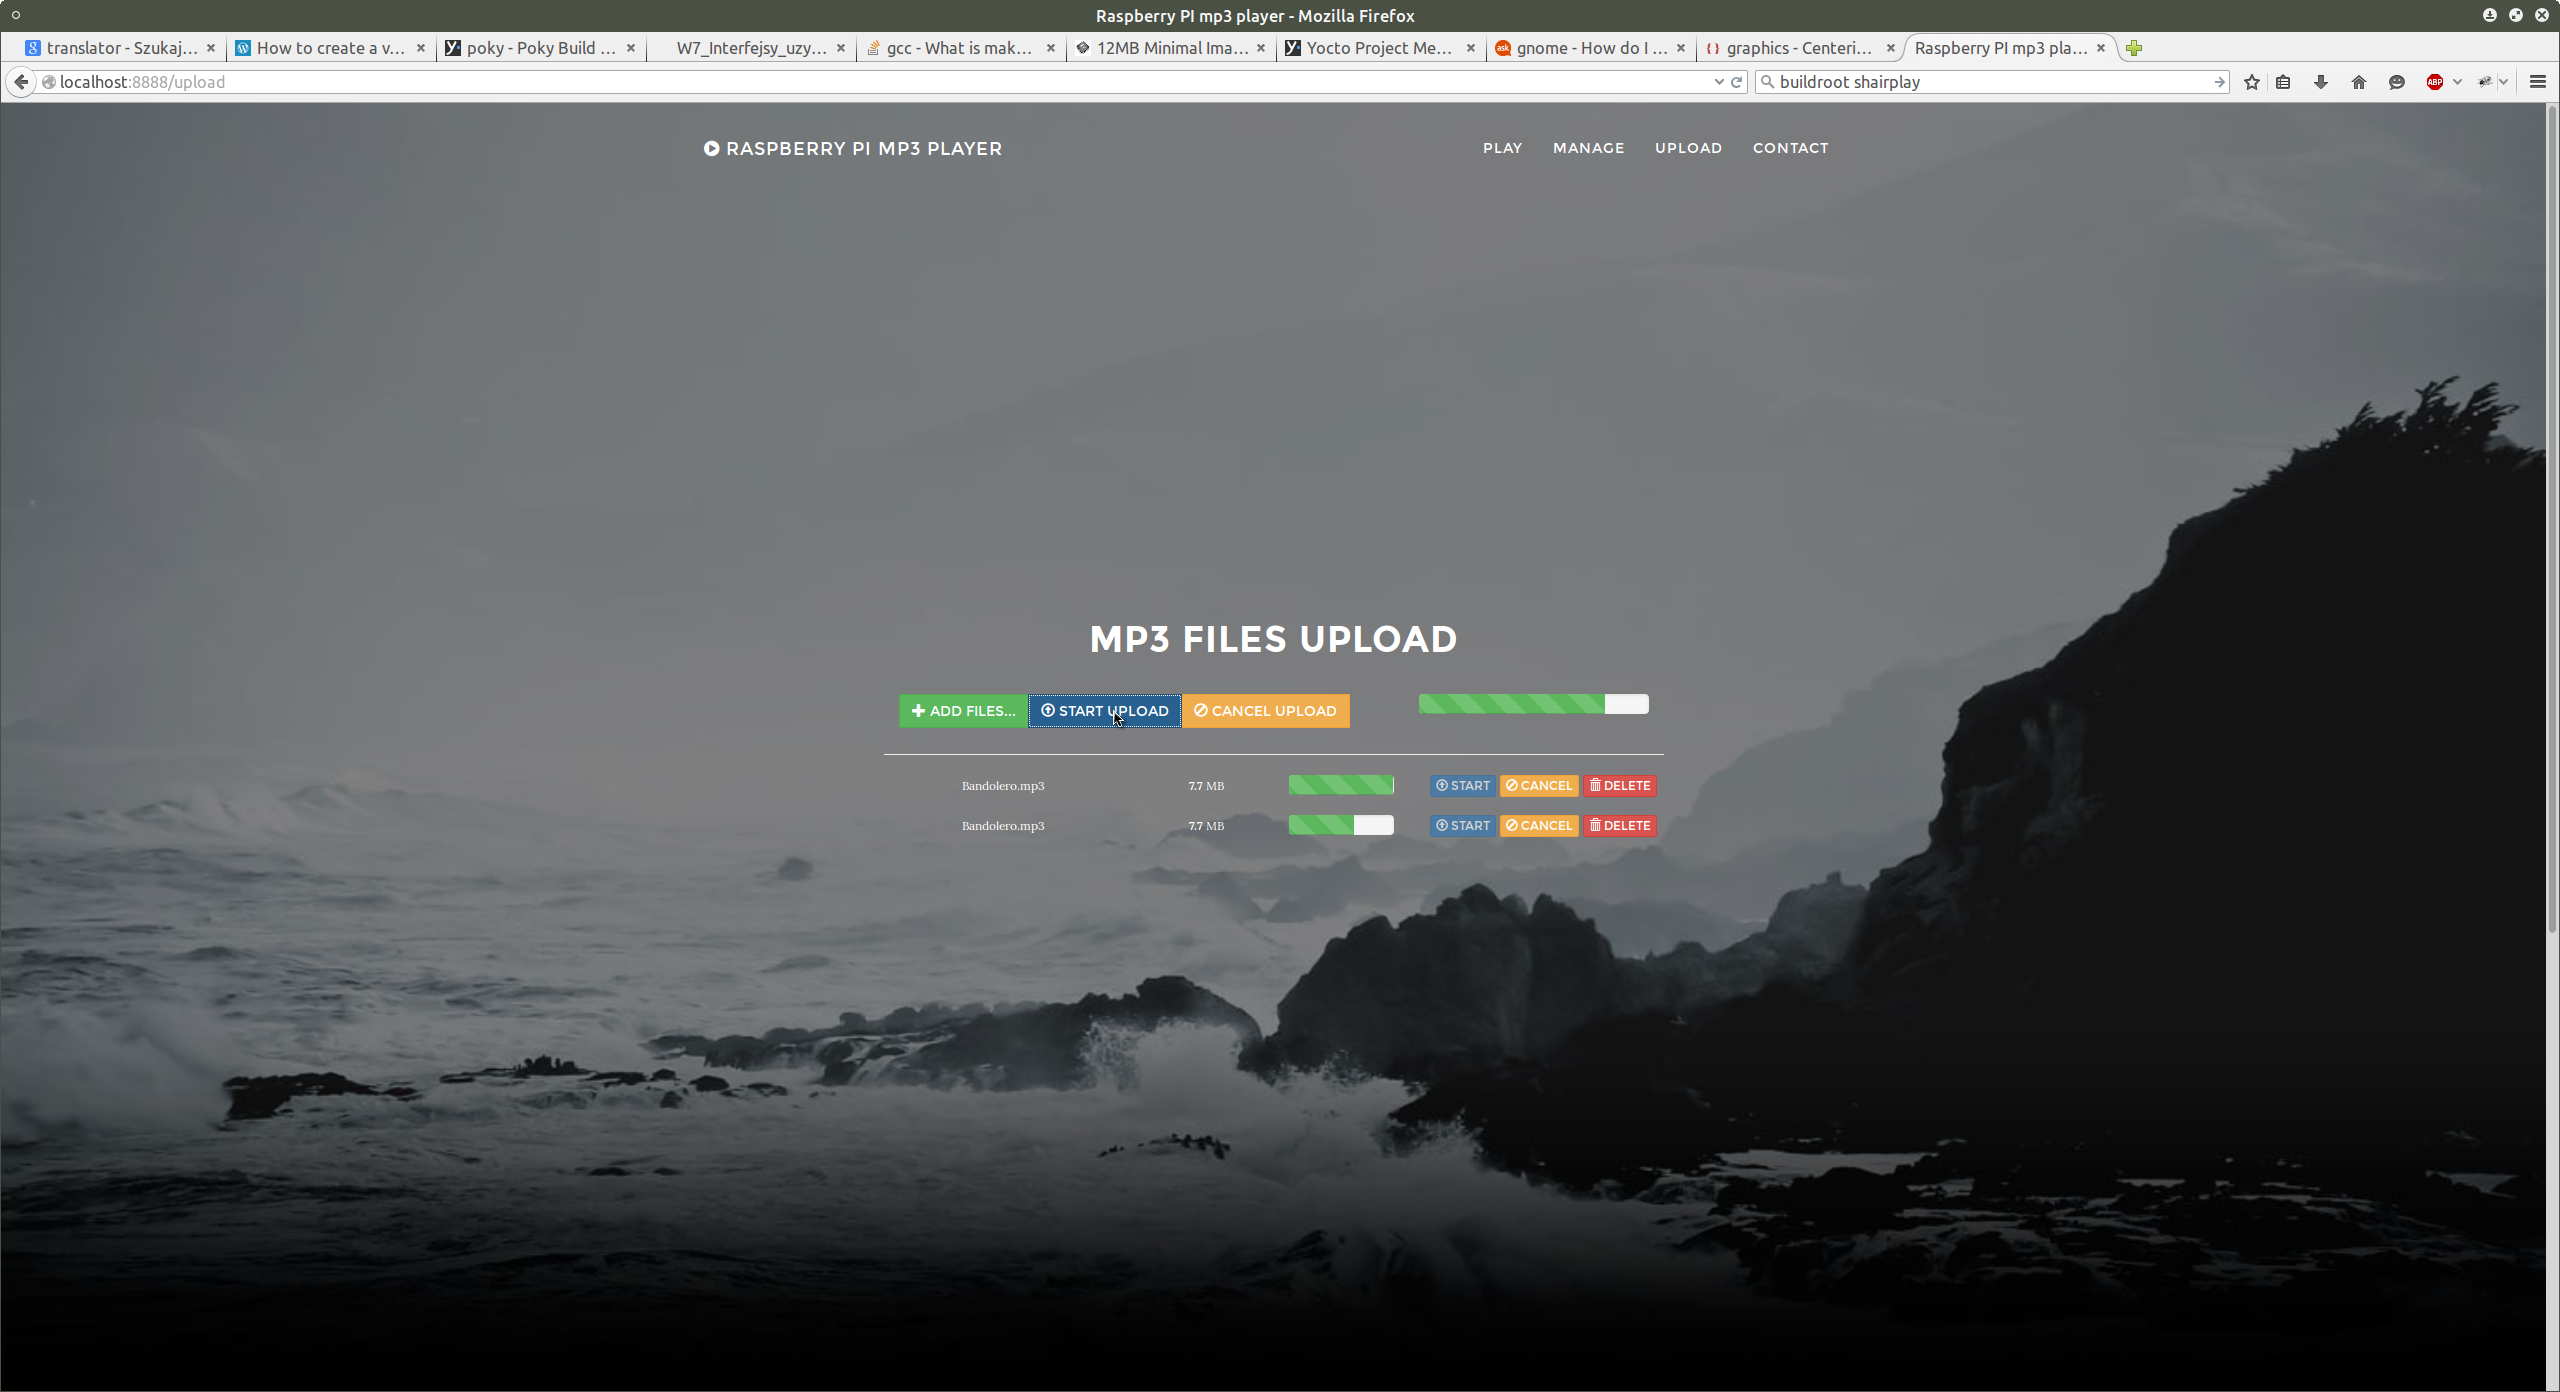
\includegraphics[width=0.75\textwidth]{Upload.png}
\end{center}
\begin{center}

\includegraphics[width=0.75\textwidth]{Play.png}
\end{center}

\section{Pliki konfiguracyjne i źródła}
Pliki konfiguracyjne i źródła do tego jak i wcześniejszych zadań umieściłem w repozytorium
git na serwisie www.github.com. Aby ściągnąć te źródła należy w katalogu docelowym wykonać polecenie:
\begin{lstlisting}[language=bash]
git clone https://github.com/dzitkowskik/buildroot-rpi-linsw.git
\end{lstlisting}	
\begin{itemize}
\item buildroot\_adm\_conf -- pliki konfiguracyjne do systemu administracyjnego na initramfs
\item buildroot\_user\_conf -- pliki systemu użytkownika z systemem plików $ext4$
\item server -- pliki serwera strony internetowej w tornado (odtwarzacz muzyki) (user: admin, hasło: admin - do uploadu plików); należy skopiować ten katalog na partycję na RPI i uruchomić plik wykonywalny server.py; serwer
domyślnie powinien być uruchomiony na porcie 8888.
\item scripts -- skrypty (init - skrypt startowy dla barebox, update.sh - skrypt shellowy do aktualizacji systemu plików $e2fs$ na partycji dla użytkownika)
\item docs -- dokumentacja
\end{itemize}
\end{document}
